\chapter{Radiative Processes}
\subsection{Decription}

The analysis of the radiative processes is related to the analysis of the general scattering process. So we have briefly touched scattering in the previous section.l

Typically for the scattering processes at this level, we can distinguish between the radiative and non-radiative processes. 

Following \cite{ZygelmanCT} we consider a positively charged Hydrogen ion approaching a neutral Hydrogen atom. As the values or R (internuclear distance) becomes smaller, there increases a probability that the electron will escape one atom and attach itself to another.\\
When this happens a charge transfer has occured. \\
There are two classes of transfer, endoergic and exothermic .\\
In the endoergic case the binding energy of the electron on the ion is less than that of the atom. In this case,in order to satisfy the energy conservation requirements, an incoming ion needs to supply the additional energy. However if the ion approaches slowly, there is no extra supply of energy. So when an additional energy is not available, charge transfer can only occur if the final electron binding energy is greater than or equal to its binding energy on the atom.\\
If the energy is equal, the reaction is called resonant charge transfer.\\
if not the reaction will processed with the possibility of the emission of a photon.
If radiation is emitted, we call the reaction radiative charge transfer/association and, if not, direct charge transfer.

Radiative processes involve emission of a photon and they typically mean Radiative Charge Transfer: \\
$ A(n+1\prescript{1}{}S) + B \longleftrightarrow A(n\prescript{1}{}S) + B + \hbar\omega $ \\
and Radiative Association: \\
$ A(n+1\prescript{1}{}S) + B \longleftrightarrow A(n\prescript{1}{}S)B + \hbar\omega $ .\\
For example, the simplest case of the radiative process is the collision of the two hydrogen atoms, in the process $ H + H^+ \rightarrow H^+ + H + \hbar\omega $.\\

While the non-radiative process, with no photon emission, is a Charge Transfer: \\
$ A(n+1\prescript{1}{}S) + B(n\prescript{1}{}S) \longleftrightarrow  A(n\prescript{1}{}S) + B(n+1\prescript{1}{}S) $ .\\

Radiative Quenching is an interaction between two atoms (or molecules), one being in excited state and the other in 'normal' ground state. During this process the excited atom emits a photon and drops to a ground state.
The simplest such case is the collision of the two hydrogen molecules, in the process $ H(2\,{}^2\!S) + H(1\,{}^2\!S) \rightarrow H(1\,{}^2\!S) + H(1\,{}^2\!S) + \hbar\omega $.

There are several theoretical approaches to this problem. \cite{RadQuench1}, \cite{RadQuench2}, \cite{Zygelman88}. While the problem has not been solved analytically, we will show that it can be solved numerically, to a desired precision. The radiative processes are driven by the interaction of the collision system with the radiation field. The direct change transfer is due to the transition between atomic (molecular) states due to the nuclear motion. Because the collision energy considered is low, typically only molecular states included are those which correspond to the initial $ A \prescript{1}{}\Sigma^+ $  and final $ X \prescript{1}{}\Sigma^+ $ channels.

Here we shall investigate the low energy collision process between the hydrogen atom and the hydrogen ion, in 2 dimension. We use fully quantum mechanical approach to calculate the cross section and the emission spectra of the reaction $ H(2\prescript{2}{}S) + H(1\prescript{1}{}S)\rightarrow H(1\prescript{1}{}S) + H(1\prescript{1}{}S) + \hbar\omega $, formed by the quenching of the excited $ H $ atom by the approaching $ H $ atom, in 2D dimensions. To my knowledge, there is no experimental results related to the 2D problem. There are results for the 3D case, listed in \cite{Zygelman88} and references there.

In this calculation, the atoms are confined in 2 dimensions, while the radiation is emitted or absorbed in all 3D space. Therefore the photon can be emitted in any direction and the potential felt by the incoming ion is the standard 3D Coulomb potential.

We will model this as a scattering problem, using a Born-Oppenheimer approximation and optical theorem. The Hamiltonian in this case will contain another term, namely the interaction of the radiation field with the electron

\subsubsection{Applications}

These type of reactions often occur in the astrophysical processes. They are generators of X-rays in in astrophysical processes. They also generate X-rays in stellar environments, atmospheric environments and the interstellar mediums. Spectroscopic analysis of the spectral lines allows us to probe such environments. \\
The other application of the charge transfer is examining the behaviour of low-temperature edge plasmas in laboratory fusion device.


\subsection*{Length gauge}

This is an interesting approach, which could potentially be used in calculation. In this thesis we would nit be using it.

The length gauge is a gauge transformation that replaces the vector potential for the field by the scalar potential for the quasi-static electric field \cite{LengthGauge3}.  In this gauge we take the Hamiltonian as: $ H = \mathbf{p}^2/2m + V(\mathbf{r})  + e\mathbf{E}\mathbf{r} $. The length gauge is convenient since both the Coulomb and the external fields are represented by the scalar potentials, which are additive. In the presence of the radiation field, the length gauge is obtained by the gauge transformation of the vector potential $ \mathbf{A} $, such that $ \mathbf{A} \rightarrow \mathbf{A} + \nabla \chi $ where $ \chi = - \mathbf{r} \cdot \mathbf{A} $. 

In the length gauge, the interaction Hamiltonian is:
\begin{equation}
\begin{split}
& H_{int} = -\sum_j{ \mathbf{r}\cdot\mathbf{E} } \\[.8em]
& \mathbf{E} = i\,\sum_{k\alpha}{\left(\frac{2\pi c k}{V}\right)^{1/2}\hat{\epsilon}_{k\alpha}\left(a_{k\alpha} - a^{\dagger}_{k\alpha}\right)}
\end{split}
\end{equation}
where $ a_{k\alpha} $ and $ a^{\dagger}_{k\alpha} $ are destruction and creation operators for the photon of momentum $ \hbar k $ and polarization $ \alpha $ respectively.


In our calcution we use the Born-Oppenheimer approximation to compute the charge transfers

\subsection{Application of the Born-Oppenheimer (BO) approximation}

Following \cite{Zygelman89}  employ the Born-Oppenheimer (BO) approximation. We expand the scattering wave function in the terms of BO wave functions, adding the electronic translation factor.
If we set $ \chi_i^a(\mathbf{R}) $ to the be wave function of the nuclear motion in the electronic state $ i $, we get for the wavefunction:
\begin{equation}
\Psi(\mathbf{r},\mathbf{R}) = \sum_i{exp\left[\frac{1}{\mu}\mathbf{S}\cdot\nabla_R \right]\phi(\mathbf{r},\mathbf{R}) }\chi_i^a(\mathbf{R})
\end{equation}
with $ \mu $ being the reduced mass, and
\begin{equation}
S = \frac{1}{2}f_i(\mathbf{r},\mathbf{R})\mathbf{r}
\end{equation}
where $ f_i $s are the switching functions that incorporate the molecular character of the ETF.
The equations for the $ \chi_i^a(\mathbf{R}) $ can be obtained in a matrix form:
\begin{equation}
\left\{-\frac{1}{2\mu}\left[\underline{I}\nabla_R - i(\underline{\mathbf{P}} + \underline{\mathbf{A}})\right]^2 + \underline{V}\right\}\underline{\chi}^a(\mathbf{R}) = E\underline{\chi}^a(\mathbf{R})
\end{equation}
with:
\begin{equation}\label{matrixFactors1}
\begin{split}
& \mathbf{P}_{ij} = \Braket{\phi_i | -i\nabla_R | \phi_j} \\*
& \mathbf{A}_{ij} = i(E_i - E_j)\Braket{\phi_i | \mathbf{S} | \phi_j} \\*
& V_{ij}(R) = \delta_{ij}V_i(R)
\end{split}
\end{equation}
where $ E $ is the energy of the nuclear motion in the center of mass frame, and $ \underline{I} $ is the identity matrix. The matrix $ \mathbf{P}_{ij} $ represents the non-adiabatic coupling, the $ \mathbf{A}_{ij} $ is the ETF correction, and the $ V_i(R) $ is the potential energy of the $ i $th Born-Oppenheimer state.



Here is the Mathematica plot of the potential curves from the 2 nuclei. This is 

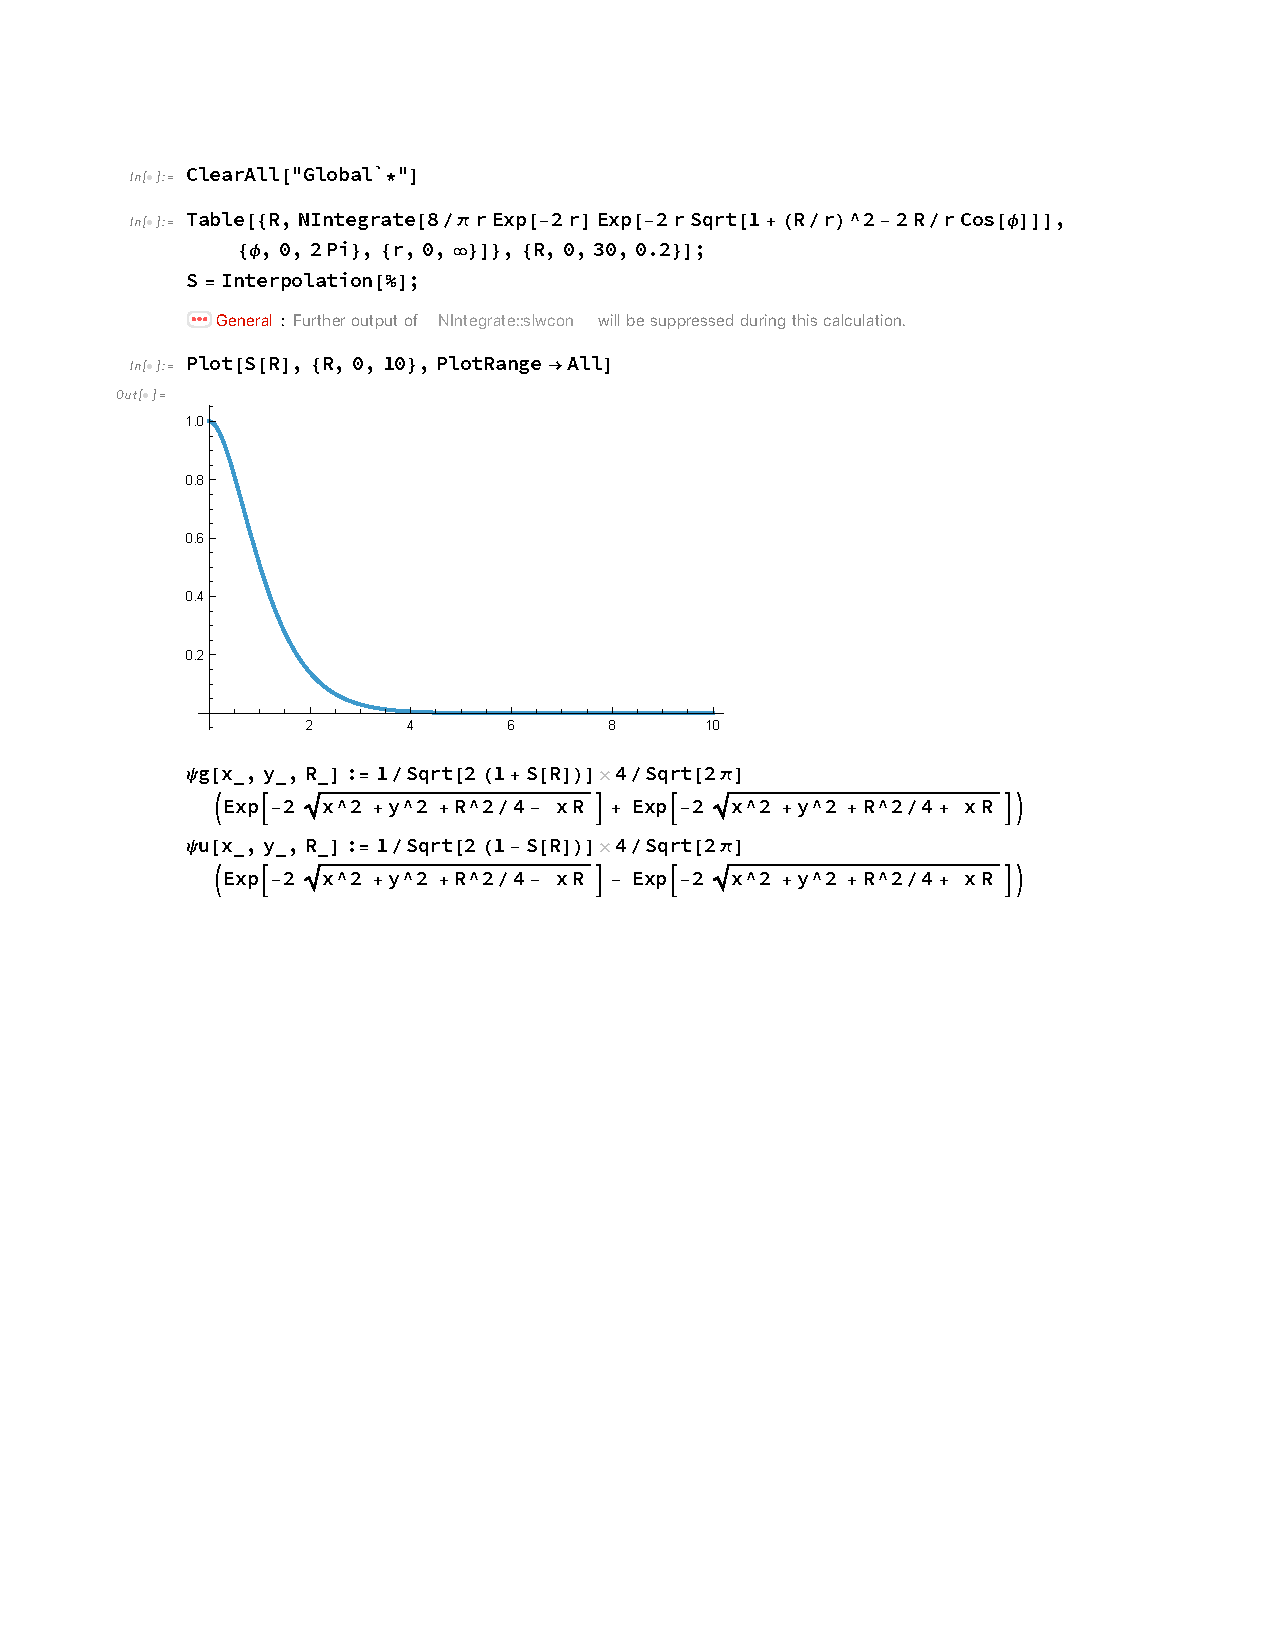
\includepdf[pages=-]{Vgraph.pdf}

\chapter{The Radiative Quenching \texorpdfstring{$ H_2^+ $}{$H_2^+$}  Ion Atom Collisions in 2D Space} 
\label{chp:quenching}

\section{Radiative Quenching Analytical Analysis}

We start with the following Hamiltonian.
\begin{equation}\label{eqH1} 
\begin{split} 
& H = -\frac{1}{2\mu}\nabla^2_{\mathbf{R}} + H_{el}(\mathbf{R},\mathbf{r}) + H_{rad} + H_{int} 
\end{split} 
\end{equation} 

where $ \mu = \frac{m_p\,m_e}{m_p + m_e} $, is the reduced mass, $ \nabla_{\mathbf{R}} $ is the gradient operator for the relative nuclear motion. $ H_{el}(\mathbf{R},\mathbf{r}) $ is the fixed nuclei Hamiltonian for the electron, whose coordinate are labeled by $ \mathbf{r} $. $ H_{rad} $ is the Hamiltonian of the radiation field, and $ H_{int} $ is the radiation-matter coupling. Since we are dealing with the interaction of an atom with the EM radiation, it is common to use the length gauge.  

So if we regard this process as a transition induced by the radiation field from the $ A^{1}\Sigma^{+}_u $ state to of the $ H_2 $ molecule formed by the approaching $ H $ atom, to the $ X^{1}\Sigma^{+}_g $ state in which the atoms separate.

Now given the Hamiltonian for the homonuclear diatom with one electron:
\begin{equation}\label{hdia}
  H = -\frac{1}{2}\vec{\nabla}^2 + V_a(\vec{r} - \frac{\vec{R}}{2}) + V_b(\vec{r} + \frac{\vec{R}}{2}) + V(|\vec{R}|) 
\end{equation}
where $ V_a, V_b $ are the electron nucleus Coulomb interaction for the nuclei A and B respectively. The $ \vec{r} $ is the position of the electron and $ \vec{R} $ is the distance between the nuclei.

Asymptotically, for large $ |R| $ we have for the Hamiltonian and eigenstates:
\begin{equation}
\begin{split} 
  & H_a = -\frac{1}{2}\vec{\nabla}^2 + V_a(\vec{r} - \frac{\vec{R}}{2}) \text{ with the eigenstate: } \Phi_a(\vec{r} - \frac{\vec{R}}{2}) F_a(R) \\
  & \text{and} \\
  & H_b = -\frac{1}{2}\vec{\nabla}^2 + V_b(\vec{r} + \frac{\vec{R}}{2}) \text{ with the eigenstate: } \Phi_b(\vec{r} + \frac{\vec{R}}{2}) F_b(R) \\
\end{split} 
\end{equation}

From the physics of the system, we have two classes of solution, Gerade and Ungerade. Those correspond to the parity of the electron's wavefunction.

So following the \cite{Dalgarno1953} we have the $ |R| \rightarrow \infty $ asymptotic eigenstates of equation \eqref{hdia}, both gerade and ungerade:
\begin{equation}
\begin{split}
  & \Phi_g = \frac{1}{\sqrt{2}}\left(\Phi_a(\vec{r} - \frac{\vec{R}}{2}) + \Phi_b(\vec{r} + \frac{\vec{R}}{2})\right) \\
  & \Phi_u = \frac{1}{\sqrt{2}}\left(\Phi_a(\vec{r} - \frac{\vec{R}}{2}) - \Phi_b(\vec{r} + \frac{\vec{R}}{2})\right) 
\end{split}
\end{equation}

So we now apply the scattering analysis for 2D, from the previous chapter, and assume that $ F_g(r) $ at asymptotic distances obeys the 2D conditions:
\begin{equation}
  F_g(R) \underset{R \rightarrow +\infty}{\sim} e^{ik\ x} + f_g(\theta)\frac{e^{ik\ x}}{\sqrt{R}} 
\end{equation}
Now we use the 2D scattering amplitude from the previous chapter:
\begin{equation}\label{fgampl}
  f_g(\theta) = \sqrt{\frac{2}{Pi}}\sum_{m=0}^{\infty}{\epsilon_m \cos(m\theta)e^{i\delta_m^g}\sin\delta_m}
\end{equation}
As the $ f(\theta) $ is not directly observable, in 2D we look for the scattering length. And we get for the scattering length, in 2D:
\begin{equation}
\begin{split}
  & \theta_g = \int_{0}^{2Pi}{d\theta f_g(\theta)} = \frac{2}{Pi}\sum_{m,m'}\int_{0}^{2Pi}{\epsilon_m\epsilon_m' \cos(m\theta)\cos(m'\theta)e^{i\delta_{m}^g}e^{i\delta_{m'}^g}\sin\delta_m^g\delta_{m'}^g} = \\
  & = \frac{2}{Pi}\sum_{m}{\epsilon_m\sin^2\delta_m^g}
\end{split}
\end{equation}
The same discussion applies for the ungerade solution so we :
\begin{equation}
  \theta_u = \frac{2}{Pi}\sum_{m}{\epsilon_m\sin^2\delta_m^u}
\end{equation}

In our case we are not interested in the elastic scattering of the gerade and ungerade states,as they form the linear combination of the asymptotic orbitals for the atom A and B, respectively.

Instead we seek the asymptotic form for the difference
\begin{equation}
  \frac{1}{2}\left(F_g(R) - F_u(R)\right) \sim \frac{\left|f_g(\theta) - f_u(\theta)\right|}{4Pi}
\end{equation}
Using expression \eqref{fgampl} we get:
\begin{equation}
\begin{split}
  & theta = \frac{1}{4}\int_{0}^{2Pi}d\theta\frac{\left|f_g(\theta) - f_u(\theta)\right|^2}{4Pi} \Rightarrow \\ 
  &  theta = \frac{1}{k}\sum_{m}\epsilon_m\sin^2(\delta_u-\delta_g)
\end{split}
\end{equation}

Now we write the system wave function:
\begin{equation}\label{ansatzWave1}
\Ket{\Psi} = F_a(\mathbf{R})\chi_a(\mathbf{R},\mathbf{r})\Ket{0} + \sum_{k\alpha}{F_{k\alpha}(\mathbf{R})\chi_b(\mathbf{R},\mathbf{r})\Ket{k\alpha}}
\end{equation}

where $ \chi_a(\mathbf{R},\mathbf{r}) $ and $ \chi_b(\mathbf{R},\mathbf{r}) $ are the eigenstates of the fixed position nuclei Hamiltonian $ H_{el} $ corresponding to the $ A^{1}\Sigma^{+}_u $  and $ X^{1}\Sigma^{+}_g $ state in body fixed frame respectively. The $ F_a(\mathbf{R}) $ and $ F_{k\alpha}(\mathbf{R}) $ are the amplitudes for the relative nuclear motion and $ \Ket{0} $ and $ \Ket{k\alpha} $ are the kets for the photon vacuum and single photon states. The ansatz \eqref{ansatzWave1} is valid at low speed collisions, where the other channels are inaccessible. In the adiabatic approximation (i.e. ignoring the non-adiabatic effects) the amplitudes $ F_a(\mathbf{R}) $ and $ F_{k\alpha}(\mathbf{R}) $ obey the set of coupled equations:
\begin{equation}\label{Fk}
\begin{split}
& \left[-\frac{1}{2\mu}\nabla^2_{R} + V_a(R) - E\right]F_a(\mathbf{R}) = \sum_{k\alpha}{F_{k\alpha}(\mathbf{R})U_{k\alpha}(\mathbf{R}) } \\[.8em]
\end{split}
\end{equation}
\begin{equation}\label{Fka}
\begin{split}
& \left[-\frac{1}{2\mu}\nabla^2_{R} + V_b(R) + \hbar\omega - E\right]F_{k\alpha}(\mathbf{R}) = F_a(\mathbf{R})U^{\dagger}_{k\alpha}(\mathbf{R}) 
\end{split}
\end{equation}
where
\begin{equation}
\begin{split}
U_{k\alpha}(\mathbf{R}) = -i\left[\frac{2\pi c k}{V}\right]^{1/2}D(R)\hat{\mathbf{R}}\cdot\hat{\mathbf{\epsilon}}_{k\alpha}
\end{split}
\end{equation}
and $ V_a(R), V_b(R) $ are the potential energy curves for the $ A^{1}\Sigma^{+}_u $ and $ X^{1}\Sigma^{+}_g $ states respectively.   $ D(R) $ is the radial transitional dipole moment between them. $ E $ is the initial energy of the relative motions and $ \omega $ is the angular frequency of the emitted photon. 
Now the next step is to solve this. We find the Green function for the equation \eqref{Fka} which satisfies the retarded boundary conditions so that $ F_{k\alpha} $ contains only outgoing waves in the limit $ R \rightarrow \infty $:
\begin{equation}\label{GreenFkaEq1}
\begin{split}
& \left[-\frac{1}{2\mu}\nabla^2_{R} + V_b(R) + \hbar\omega - E\right]G^{+}(\mathbf{R}, \mathbf{R}') =  \delta^3(\mathbf{R}, \mathbf{R}')
\end{split}
\end{equation}
and from the equation \eqref{GreenFkaEq1} we get:
\begin{equation}\label{FkaInt1}
\begin{split}
& F_{k\alpha}(\mathbf{R}) = \int{d^3R'G^{+}(\mathbf{R}, \mathbf{R}')F_{a}(\mathbf{R}')U^{\dagger}_{k\alpha}(\mathbf{R}')   }
\end{split}
\end{equation}

\section{Solution Strategies}
The main approaches to solving problems is to expand the wave function in the partial waves basis and use Born approximation.

Using partial waves  we expand the incoming wave in the basis of spherical harmonics, and in the case of azimuthal symmetry to the basis of Legendre Polynomials. This in effect mean that we decompose each wave into its constituent angular momentum components and solving using boundary conditions.

Born approximation \cite{GQuantum} treats a scattering potential as a perturbation to the incoming wave. In this case many partial waves contribute to scattering, so it is preferable to avoid angular momentum decomposition. The Born approximation is generally applicable either when the energy of the incoming particle(s) is high or when the scattering potential is very weak. 

\subsection{Using Partial Waves}

Again we write the time independent Schroedinger equation in 2D:
\begin{equation}
  -\frac{1}{2}\nabla^2\psi + V\psi = E\,\psi
\end{equation}

where m is the reduced mass, V is a short-range local potential, E is the relative energy.

Using polar coordinates, setting $ k^2 = 2mE $ , we have the equation
\begin{equation}
    \frac{1}{r}\frac{\partial}{\partial r}\left(r\frac{\partial\psi(r\theta)}{\partial r}\right) + \frac{1}{r^2}
\end{equation}

We expand the incoming wave in the partial wave basis as:
\begin{equation}
    e^{ikx} = e^{ikr\cos\theta} = \sum_{m=0}^{\infty}{\epsilon_m \cos(m\theta)J_m(kr)}
\end{equation}
where $\epsilon_m = 2 $ for $ m \ne 0 $ and $\epsilon_0 = 12 $.


We define a scattering length in 2 dimensions,, analogous to the scattering cross section in 3D, as:
\begin{equation}\label{scatterL}
  \lambda(\theta) = |\sqrt{\frac{i}{k}}f_f(\theta)|^2
\end{equation}

The equation \eqref{scstterL} represents the number of particles scattered between $ \theta $ and $ \theta + d\theta $ per second per unit incident flux.

We can express this function in the partial waves bases. Since $ V_b $ contains no bound states we get for $ \mathbf{R} = \mathbf{R}(R,\theta) $:
\begin{equation}\label{GreenFka2}
\begin{split}
G^{+}(\mathbf{R}, \mathbf{R}') =  \frac{\pi\mu}{k_b}\sum_{l=0}^{\infty}{\sqrt{\frac{1}{2\pi}} P_l(\cos\theta) P_l^{*}(\cos\theta^{'})}\times \frac{f_l(k_bR_{<})g^{+}_l(k_bR_{>})}{RR'}
\end{split}
\end{equation}
where $ P_l(\cos\theta) $ are Legendre polynomials, also $ \theta = 0 $ part of the spherical harmonics:  $ P_l(\cos\theta) = Y_{l0}{\theta,0} $. 

The $ f_l(R) $ is a regular solution of the homogeneous Schrodinger radial  equation for the 2D case: \cite{H2atom}:
\begin{equation}\label{eqRadial1}
\begin{split}
  & \frac{1}{R}\frac{d}{dR}\left(R \frac{d}{dR}\,f_m(R)\right) + \left\{k^2 - \frac{m^2}{R^2} - 2\mu\left[V_b(R) - V_b(\infty)\right] \right\}f_m(R) = 0 \\[.8em]
& k \equiv \sqrt{2\mu[E - \hbar\omega - V_b(\infty)}
\end{split}
\end{equation}
where:
The solution of the equation \eqref{eqRadial1} are Bessel functions $ J_m(kR) $ and $ N_m(kR) $ with the asymptotic behaviour:
\begin{equation}
\begin{split}
f_{m}(kR)\sim \sqrt{\frac{2}{\pi kR}}\cos\left[kR - \pi\frac{m+1/2}{2} \right],\,\,{R \rightarrow \infty}
\end{split}
\end{equation}
and $ g^{+}_l(kR) $ is irregular solution with the boundary condition at large $ R $.
\begin{equation}\label{remoteWave}
\begin{split}
g^{+}_{m}{(kR)} \sim \sqrt{\frac{2}{\pi kR}}\cos\left[kR - \pi\frac{m+1/2}{2} + \delta_m\right],\,\,{R \rightarrow \infty}
\end{split}
\end{equation}
and $  \delta_m $ is a phase shift. 

The total wave function \eqref{ansatzWave1} must be symmetric under the interchange of the $ H $ nuclei, so that $ F_a(\mathbf{R}) = -F_a(-\mathbf{R}) $ and $ F_{k\alpha}(\mathbf{R}) =  F_{k\alpha}(-\mathbf{R}) $. Now we solve equations \eqref{Fk} and \eqref{Fka} in the distorted wave approximation. Then $ F_a(\mathbf{R}) $ is the solution of the \eqref{Fk} with the coupling term set to be zero and it can be expressed in the form:
\begin{equation}\label{Flong1}
F_a(\mathbf{R}) = \sum_{m=1}^{\infty}{P_m(\cos\theta)(2m+1)i^{l}\sqrt{\pi}\times \exp[i\delta_m]\frac{s_m(k_a\mathbf{R})}{k_a\mathbf{R} } } 
\end{equation}

The asymptotic form for \eqref{Flong1} is:
\begin{equation}\label{FlongA}
F_a(\mathbf{R}) \sim \frac{1}{\sqrt{2}}\left[e^{ik_az}-e^{-ik_az} + [f(\theta,\phi) - f(\theta-\pi,\phi+\pi)]\frac{e^{ik_aR}}{R}\right]
\end{equation}

By inserting \eqref{Flong1} and \eqref{GreenFka2} into \eqref{FkaInt1} we get the asymptotic form for the  \eqref{FkaInt1}:
\begin{equation}\label{FlongAA1}
F_{k\alpha}(\mathbf{R}) \sim \frac{e^{ik_aR}}{R}f_{k\alpha}(\theta)
\end{equation}
where:
\begin{equation}\label{fkaa1}
f_{k\alpha}(\theta) = \sum_{m}{\cos(l\,\theta)\left[\sum_{m=1}^{\infty}{\frac{2\pi\mu}{k_ak_b}(2m+1)\left(\frac{\pi k c}{A}\right)^{1/2}e^{i\delta_j(b)}e^{i\delta_j(a)}i^{J+l-1} }\right]\sqrt{2l+1)2\pi}}
\end{equation}

In this summation, the $ j $ is restricted to the odd integers, and 
\begin{equation}\label{Mll1}
M_{m,m'}(k_a,k_b) = \frac{1}{\sqrt{k_a,k_b}}\int_0^{\infty}{dRs_m(k_a,R)D(R)f_{m'}(k_b,R)} 
\end{equation}

The cross section of the collision induced transition between the $ H $ atom and the $ H^{+} $ ion is obtained by summing $ \left|f_{k\alpha}(\theta)\right|^2 $ over all final states that conserve energy with an initial state, and dividing the result with the flux of the incident channel.

The $ H\left(2 \leftidx{^1}{}S\right) \rightarrow H\left(1 \leftidx{^1}{}S\right) $ is a linear combination of $ A \leftidx{1}{}\sigma_u^{+} $ and $ X \leftidx{1}{}\sigma_g^{+} $ states. Since the excited gerade state is not allowed to make a radiative transition to a gerade ground state, the flux in the incident channel is twice the flux in the $ A \leftidx{1}{\sigma_u^{+}} $ channel.

So for the scattering length we get:
\begin{equation}\label{crs1}
\begin{split}
& \sigma = \int_0^{\omega_{max}}{d\omega\frac{d\sigma}{d\omega}} = \\[.8em]
& = \sum_{\alpha}{\int{\frac{d^2k}{(2\pi)^2}\frac{A}{2\mu k_a}\int{d^2k_b\delta\left[\frac{k_b^2}{2\mu} - \frac{k_a^2}{2\mu} + \Delta E - \hbar\omega \right]\left|f_{k\alpha}(\theta) \right| } } }
\end{split}
\end{equation}

where
\begin{equation}\label{diffcrs1}
\frac{d\sigma}{d\omega} = \frac{8}{3}\left[\frac{\pi \mu}{k_a}\right]^2 \frac{1}{c^3}\omega^3 \sum_{J}{\left[J M_{J,J-1}^2(k_a,k_b) + (J+1)M_{J,J+1}(k_a,k_b)\right] }
\end{equation}

$ \Delta E $ is the energy of the transition at $ R = \infty $ and $ \omega_{max} $ is the maximum frequency of the emitted photon. Expression \eqref{crs1} is an equivalent expression to the Fermi's Golden Rule. Equation \eqref{diffcrs1} provides the spectrum of the emitted radiation, in addition to the scattering cross section. 

\subsection{Phase Shift Calculation}

\begin{equation}
\begin{split}
  \lambda = \frac{4}{k}\sum_{m=0}^{\infty}{sin^2(\delta_m^{+}-\delta_m^{-})}
\end{split}
\end{equation}

It is now fairly straightforward to compute the scattering length. We compute the scattering length in the Wolfram Mathematica code listed in appendix E.

The following is the plot of the scattering length in a.u. vs temperature in Kelvin.

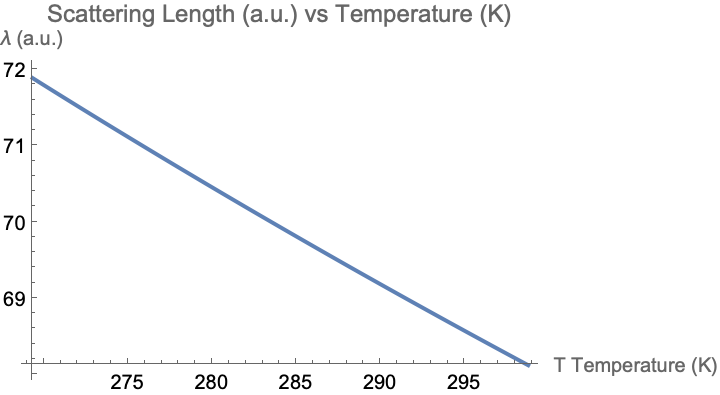
\includegraphics{CrossSection1.png}

\subsection{Optical Potential Method, Dipole Moment and Einstein A Coefficient}

The approximation that does not require the integration over the total spectrum is the optical potential method. 

Again it is assumed that the scattering takes place at low energies, so that the system can be described by a wave function $ \Psi(x,t) $ which is itself a solution of a Schrodinger equation $ H\ket{\Psi(t)} = i\hbar\frac{\partial}{\partial t}\ket{\Psi(t)} $ where $ H $ is a Hamiltonian $ H = T + V $ .
Then we borrow a concept from the optics, where there is a concept of a Complex Refractive Index $ n $. The real part of $ n $ describes how the light is transmitted and the imaginary part describes how the light is absorbed. So it the imaginary part that describes the effect of the scattering. We then express the potential $ V = U + iW $  and the Schrodinger equation becomes $ \left[H + U + iW\right]\ket{\Psi(t)} = i\hbar\frac{\partial}{\partial t}\ket{\Psi(t)} $. From this one gets the scattering cross section:
\begin{equation}
\sigma = \frac{k}{E}\int{d^3R\left[-W(R)\right]\left| \psi(R) \right|}
\end{equation}

To derive it here we insert the equation \eqref{FkaInt1} for the amplitude $ F_{k\alpha}(\mathbf{R}) $ into the equation \eqref{Fk} to obtain the equation for the amplitude $ F_a(\mathbf{R}) $
\begin{equation}\label{opt1}
\begin{split}
\left[-\frac{1}{2\mu}\nabla_R^2 + V_a(R) - E \right]F_a(\mathbf{R}) = \sum_{k\alpha}{d^2R'G^{+}(\mathbf{R},\mathbf{R}^{'})U_{k\alpha}^{\dagger}(\mathbf{R}^{'})U_{k\alpha}(\mathbf{R})F_a(\mathbf{R}^{'})}
\end{split}
\end{equation}

The right hand of \eqref{opt1} contains a complex, non-local potential
\begin{equation}\label{optV1}
V(\mathbf{R},\mathbf{R}^{'}) = \sum_{k\alpha}{G^{+}(\mathbf{R},\mathbf{R}^{'})U_{k\alpha}^{\dagger}(\mathbf{R}^{'})U_{k\alpha}(\mathbf{R}) }
\end{equation}

that arises because of the interaction of the electron with the vacuum. Now the real part of this potential induces the shift in the eigenvalue $ V_a(R) $. Since the coupling on an electron with the radiation is weak, we can ignore it and consider only the imaginary part. 

The imaginary part of $ V(\mathbf{R},\mathbf{R}^{'}) $ is an absorptive potential, representing a process where electron in excited state emits a photon and decays to a ground state. This potential is non-local, as we take is for $ R = \infty $. In the optical potential approximation, we take replace potential by the local one, whose range is limited to the scattering area. This potential is essentially classical.

Because the term $ U_{k\alpha}^{\dagger}(\mathbf{R}^{'})U_{k\alpha}(\mathbf{R}) $ appearing in equation \eqref{optV1} is real, the optical potential is proportional to the imaginary part of the retarded Green's function, which is expressed as:
\begin{equation}\label{OptGreen1}
\begin{split}
\text{Im} G^{+}(\mathbf{R},\mathbf{R}) = \pi\sum_{l=0}^{\infty}{\cos(l\, \theta)\cos(l\,\theta^{'})\int_0^{\infty}{dk\,\delta\left[\frac{k^2}{2\mu} - \frac{k^2_a}{2\mu} + \hbar\omega - \Delta E \right]\frac{f_l(kR)f_l(kR^{'})}{R\,R^{'}} }  }
\end{split}
\end{equation}

This result is obtained using the spectral representation of the retarded Green's function and the identity $ 1/(x + i\epsilon) \rightarrow P/x - i\pi\delta(x) $ as $ \epsilon \rightarrow 0 $. Using \eqref{OptGreen1} one obtains for the non-local optical potential:
\begin{equation}\label{optV2}
\begin{split}
&V(\mathbf{R},\mathbf{R}^{'}) = \frac{i}{2\pi}\sum_{\alpha}\int{d\Omega_k}\int_0^{k_{max}}\sum_{l=0}^{\infty}\cos(l\, \theta)\cos(l\,\theta^{'}) \\[.8em]
&\times\frac{\omega^3}{c^3}\frac{f_l(kR)f_l(kR')}{R\,R'}D(R)D(R')(\hat{\mathbf{R}}\cdot\epsilon_{k\alpha})(\hat{\mathbf{R}}^{'}\cdot\epsilon_{k\alpha})
\end{split}
\end{equation}

where $ \omega(k) = k_{\alpha}/2\mu + \Delta E - k^2/\mu $.  Now for the optical-potential approximation we make the semi-classical approximation that the values of $ k $ that give the largest contribution are given by:
\begin{equation}
\frac{k^2}{2\mu} \simeq = \Delta E + \frac{k_{\alpha}^2}{2\mu} + V_b(r) - V_a(r)
\end{equation}

Now the frequency term $ \omega^3 = \left|\Delta E(R)\right|^3 $ can now be taken outside the integral.

Using the delta function expansion in 2 dimensions: 
\begin{equation}
\delta^{(2)}\left(\mathbf{R},\mathbf{R}^{'}\right) = \sum_{l=0}^{\infty}{\cos(l\,\theta)\cos(l\,\theta')\frac{\delta(R - R')}{R\,R'}}
\end{equation}

we get:
\begin{equation}
\begin{split}
    & V_{opt}(\mathbf{R},\mathbf{R}) \approx = \frac{i}{2}\delta^{(2)}\left(\mathbf{R},\mathbf{R}^{'}\right)A(R), \\[.8em]
& A(R) = \frac{4}{3}D^2(R)\frac{\left|\Delta E(R)\right|^3}{c^3}
\end{split}
\end{equation}

and equation \eqref{optV2} becomes:
\begin{equation}\label{optApprox1}
\left[-\frac{1}{2\mu}\nabla_R^2 + V_a(R) - E\right]F_{\alpha}(\mathbf{R}) = \frac{i}{2}A(R)F_{\alpha}(\mathbf{R})
\end{equation}

The cross section for the radiative quenching is given by:
\begin{equation}
\sigma = \frac{\pi}{k_a^2}\sum_{m=0}^{\infty}{(2m+1)\left(1-e^{-4\eta_j}\right) }
\end{equation}

where $ \eta_j $ is the imaginary component of the phase shift of the $ Jth $ partial wave of the solution \eqref{optV2}. The sum on $ J $ is restricted to the odd integers. 
Also because the right hand of \eqref{optV2} is small, we can use the distorted wave approximation to obtain the expression for the phase shift $ \eta_j $
\begin{equation}\label{eta1}
\eta_j = \frac{\pi\mu}{2k_a}\int_0^{\infty}{dR\,\left|g_m^{+}\left(k_aR\right)\right|^2A(R) }
\end{equation}

\subsection{Calculation} \label{QuenchingCalculation}

We use the code in appendixE for calculating the phase shift $ \eta $, from the equation \eqref{eta1}.
First we calculate the $ D(R) $. Following \cite{DRZygelman} we have:
\begin{equation}
D(\vec{R}) = \Braket{\psi_u(\vec{r}) | (-1)\mid e \mid\,\vec{r} | \psi_g(\vec{r})} - |e|\vec{R}
\end{equation}
Where the $ \psi_g(\vec{r}) $ and $ \psi_u(\vec{r}) $ are the electron gerade and ungerade eigenstates respectively and $ \vec{r} $ is the electron coordinate. 
Because of the symmetry of the $ H_2^+ $ ion we can deduce that the dipole moment vanishes for the $ g \leftrightarrow g $ and $ u \leftrightarrow u $ transitions. This is consistent with the dipole selection rule, where allowed dipole transitions are those between states of opposite parity.

In our case, the dipole integral is:
\begin{equation}
  \int{d\xi d\eta\,L_u^*(\xi)M_u^*(\eta)\xi \eta L_g(\xi)M_g(\eta)\frac{\xi^2-\eta^2}{sqrt{\xi^2-1}\sqrt{1-\eta^2}}}
\end{equation}

Using the dipole moment we compute the Einsten A-coefficient.

Einstein A-coefficients define the probability per unit time of spontaneous emission (radiative decay) from state $ b $ to a lower state $ A $

The lifetime $ \tau = \frac{1}{A(R)} $ of an excited state is the inverse of the total A-coefficient summed over all possible downward transitions.
Knowing the dipole transition moment $ D(R) $ we can compute the Einstein $ A $ coefficient for the lowest ungerade and gerade state:
\begin{equation}
  A(R) = \frac{\pi}{\hbar\epsilon_0}D^2(R)\frac{\left|V_u(R) - V_g(R)\right|^2}{c^2}
\end{equation}

The graph of the Transition Dipole Moment between the states $ 1s^{+} $ and $ 2p^{+} $.

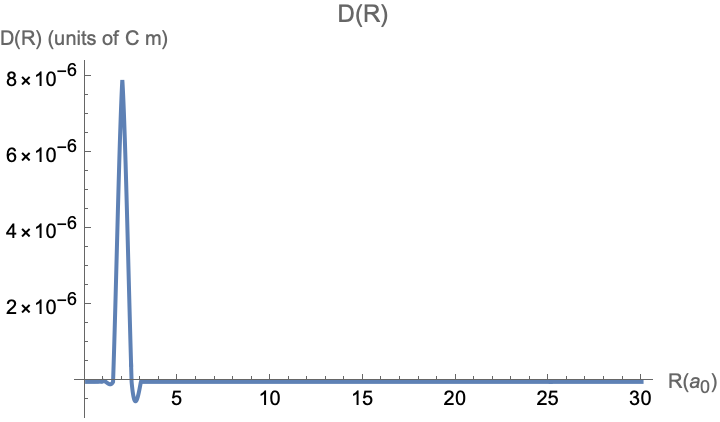
\includegraphics{DR-SI.png}

We then use transition dipole values to compute the cross section. 

The Mathematica code used for calculating the transition dipole moment  $ D(R) $ and R-dependent Einstein-A coefficient is shown n appendix F.

\subsection{Result and discussion}

Graph of the Einstein-A coefficient as function of R.

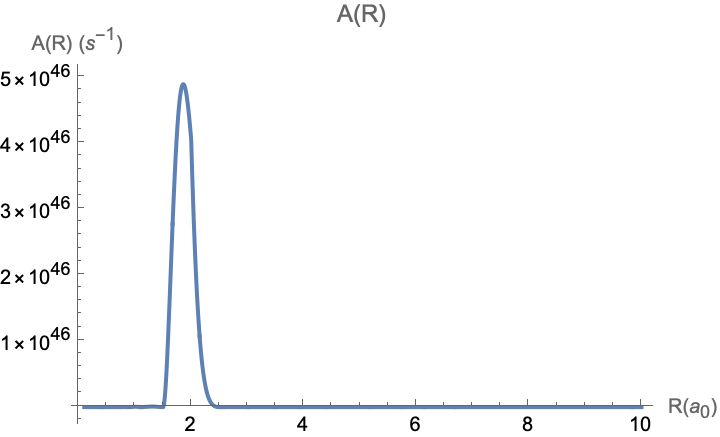
\includegraphics{AR-SI.png}

\subsubsection{Comparison with 3D case}

The paper by Dalgarno and  M R C McDowell \cite{DalgarnoMcDowel} reports that the charge transfer cross sections decrease from $ 2\times 10^{-14} cm^2 $ at an impact energy of 1 eV to $ 0.3\times 10^{-14} cm^2 $ at 1000 eV and the diffusion cross sections lead to values of the mobility of H- ions in atomic hydrogen decreasing from $ 3.5\,cm^2\,volt^{-1}\,sec^{-1} $ at 100°K to i$ 1.8\,cm^2\,volt^{-1}\,sec^{-1} $ at 600°K.

Also the paper by B. Zygelman et all \cite{ZL} in the ultra-cold limit shows values of $ A(R)$ in the order of $ 10^6\,s^{-1} $.

In our case, we observer significantly larger values $ A(R) $. This is due to two factors.

1. In 2D, the difference in potential between the gerade and ungerade states $ X^2\Sigma^+ $, $ A^2\Sigma^+ $ respectively is smaller than in the 3D case, so the probability of a transition is greater.

2. The temperature is higher in our calculation. Zygelman et all \cite{ZL} are showing that in the trickled limit the Einstein coefficients $ A(R) $ are in the order of $ 10^6\, sec^{-1} $.
